\documentclass{article}

\usepackage{graphicx}

\title{Chat application report}
\author{Abdun Nihaal}

\begin{document}
\maketitle

\section{Introduction}
The aim of this assignment is to create a chat application using java that enables users to send messages to other users one on one or in a group.

\section{Design}

\subsection{One thread per client architecture}
In this chat server architecture, whenever a client connects to the server, the server creates a separate thread to handle the client.
The problem with this architecture is that it may create more threads than what the server CPU cores can handle.
Context switching between threads can be expensive and take a lot of memory.
The client threads perform blocking reads and writes with the client.

\subsection{Selector non-blocking server architecture}
Java Nio's selector class can manage multiple channels from a single thread. 
With the use of Java Nio's selector class, I built the server which does not block when reading or writing to the client.

\begin{figure}
	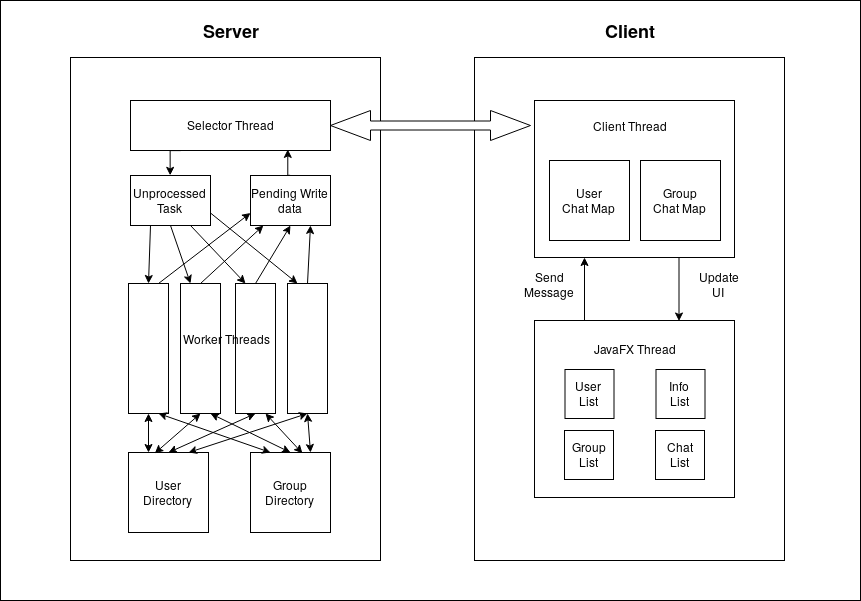
\includegraphics[width=\linewidth]{architecture.png}
	\caption{Chat server architecture}
	\label{fig:architecture}
\end{figure}

The Chat Server Architecture is shown in \ref{fig:architecture}. The server consists of a selector thread and a number of worker threads.
The selector thread is responsible for performing network IO. The worker threads process the messages that are received by the selector thread.

The communication between the selector and worker threads is achieved by using two data structures. UnprocessedTask queue is a queue of messages that were received by the selector thread. When a worker thread is free, it retrieves a message from the UnprocessedTask queue and processes it.
When the worker wants to send a message to a client, it adds the message to the PendingWrite queue. The selector thread writes the data from PendingWrite queue to the corresponding socket channel.
\section{Analysis}

\section{Results}

\end{document}
